\section{Interfaz gráfica y Jugabilidad}
El juego como ya se ha comentado consistirá en ver cómo los NPCS aplican una estrategia concreta, en este caso es el jugador el que a través de botones puede interaccionar para cambiar la estrategia. En la siguiente figura podemos ver cómo queda la interfaz
\begin{figure}[H]
    \centering
    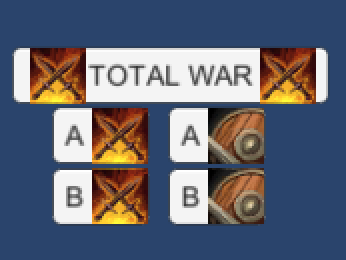
\includegraphics{buttons1.png}
    \caption{Interfaz gráfica estrategia}
    \label{fig:mainButtons}
\end{figure}
Los iconos de espadas permitirán poner el modo ofensivo al equipo que se desee mientras que el icono del escudo permite indicar al equipo que se ponga a defender. El botón de \textit{Total war} cambia el comportamiento de todas las unidades del juego para que estas den prioridad al enfrentamiento y toma de la base rival. El juego comenzará con los botones desactivados. \\

Además tendremos una segunda UI a la que accederemos \textbf{presionando la tecla \textit{I}}. Esta nos permitirá tener el minimapa de influencias en grande y el mapa de juego normal en un minimapa, teniendo la siguiente interfaz que permite cambiar el mapa que se muestra \begin{figure}[H]
    \centering
    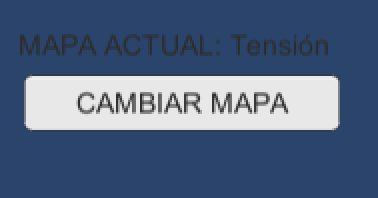
\includegraphics{buttons2.png}
    \caption{Interfaz gráfica cambio de mapa}
    \label{fig:mainButtons}
\end{figure}
